\section{Introducción}
\label{intro}
\noindent Para realizar este trabajo se ha utilizado a Baxter, un robot desarrollado por Rethink Robotics, como robot de investigación, encargado de realizar las diferentes tareas mostradas a lo largo del documento. \\

\noindent La automatización de procesos es cada vez más frecuente en la industria, es por ello que este tipo de robots seguros, que no necesitan de una infraestructura para aislarse de las personas, se utilizan. Además de la posibilidad de trabajar colaborando con un humano, son fáciles de programar, de desplazar y tienen un bajo coste comparado con el coste usual de los robots industriales.\\
Estos robots se pueden programar a través del entorno ROS, del cual se puede encontrar bastante documentación en internet, además de tener una gran comunidad, útil para consultar o solventar cualquier duda existente. \\

\begin{figure}[H]
	\centering % si queremos la imagen centrada
	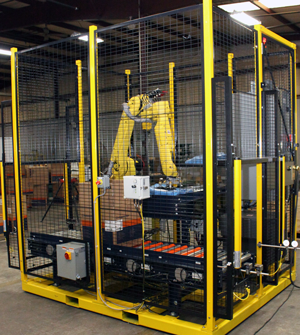
\includegraphics[scale=0.6]{imagenes/cage.png}
	\caption{Brazo robótico aislado}
\end{figure}

\noindent Como se ve en la siguiente imagen (obtenida de \cite{robgraph}), se espera que el mercado de robots industriales crezca considerablemente en los próximos años. Algunas fuentes indican que este crecimiento puede llegar a ser exponencial, llegando a aumentar de 16850 millones de dólares en 2017 a 48170 millones en 2025 \cite{robmark}. \\

\begin{figure}[H]
	\centering % si queremos la imagen centrada
	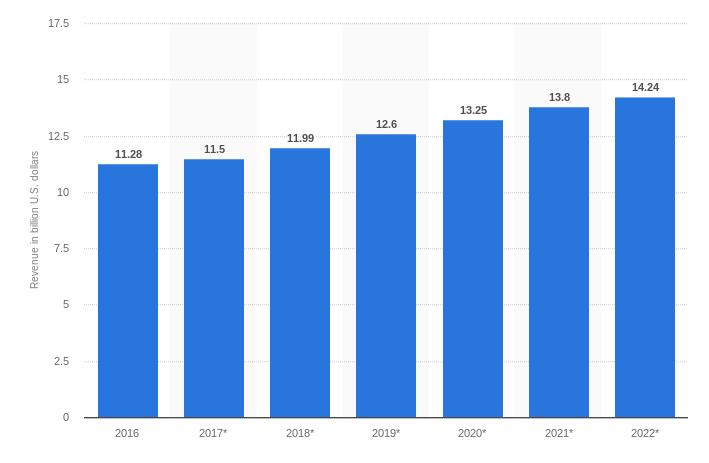
\includegraphics[scale=0.5]{imagenes/robmarket.jpg}
	\caption{Gráfica que muestra el crecimiento del mercado de robots industriales\cite{robgraph}. El eje horizontal representa el año y el eje vertical miles de millones de dólares}
\end{figure}

\noindent En este documento se explicarán las plataformas software y hardware utilizadas para realizar las tareas de clasificación de objetos con Baxter, en entorno estático y dinámico, además de realizar una comparativa de eficiencia con distintos parámetros. \\

\subsection{Motivación}
\noindent A día de hoy, en la industria existen muchos trabajos realizados por personas, a pesar de que pueden resultar peligrosos o dañinos para ellas \cite{lasota2014toward}. Debido a esto, la automatización de estas tareas resulta interesante, siendo realizadas por robots industriales que, en muchas ocasiones, suelen superar los 100000 euros.\\

\noindent En este proyecto se ha utilizado a Baxter, un robot desarrollado por Rethink Robotics, menos costoso y más seguro \cite{ju2014kinematics}, simulando una cadena de producción en la que Baxter se encarga de clasificar los objetos por color y posición, empleando el framework ROS (Robotic Operating System), MoveIt! y RViz. \\

\subsection{Situación inicial}
\noindent Como ya se ha dicho, en este proyecto se pretende realizar una clasificación de objetos en entorno estático y dinámico. Se dispone de una cinta transportadora que se utilizará en las pruebas de entorno dinámico, del robot Baxter y de las plataformas MoveIt! y RViz. Para el desarrollo de los algoritmos, se parte de un filtro de color \cite{maik}, al que se le añadirán las funcionalidades de segmentación por color y posición, planificación y ejecución de trayectorias y se realizarán distintos programas encargados de controlar a Baxter para realizar la clasificación. \\


\subsection{Objetivos}
\label{objetivos}
\noindent En este trabajo se realiza un estudio de las prestaciones de Baxter en tareas que incluyen clasificación de objetos y visión por computador. Para ello han sido fijados los siguientes objetivos:
\begin{itemize}
	\item Estudio de las funcionalidades y servicios del framework ROS.
	\item Integración de un filtro de color que permita realizar la clasificación basada en esta característica, y cálculo de grupos de objetos segmentados y recta que los separa.
	\item Desarrollo de diversos programas de clasificación de objetos y \textit{pick and place}.
	\item Clasificación de objetos según un parámetro que especifica el porcentaje de objetos de un color a obtener.
	\item Robótica adaptativa. Con la misma configuración de objetos, el esquema de control adaptará un parámetro a partir del grado de éxito de la ejecución anterior en entorno estático, lo que proporcionará cierto grado de adaptación y optimización. Este parámetro modificará el valor del brazo en el eje de ordenadas.

	\item Realización de pruebas, estudio de prestaciones y barras de error de las tareas realizadas.
	\item Liberación del software desarrollado y documentación alojados en \textit{GitHub}. Creación de una web con el contenido para que pueda ser utilizado por otros investigadores.
\end{itemize}

\subsection{Procedimiento}
\noindent Estos objetivos se pueden englobar en dos módulos, \textbf{módulo de reconocimiento}, encargado de realizar la segmentación por color y posición y enviar los datos obtenidos al \textbf{módulo de control}, cuya función será controlar a Baxter para realizar los movimientos definidos por la planificación de trayectorias. \\
\noindent Así pues, puntualizamos varias funcionalidades:

\begin{itemize}
	\item Identificación de objetos.
	\item Segmentación en dos grupos por color y posición.
	\item Obtención del punto medio entre ambos grupos de objetos.
	\item Planificación y ejecución de trayectorias.
\end{itemize}

\noindent Tras cumplir estas competencias, cada algoritmo procederá como le corresponda según tipo de entorno.

\subsection{Historia de la robótica}
\noindent El comienzo de la historia de la robótica data del 250 a. C. \cite{Robotic} En esta fecha Ctesibius de Alejandría, un físico e inventor griego, ideó una de las primeras aproximaciones de lo que hoy conocemos como autómata: el reloj de agua o \textit{clepsydra}, que medía el tiempo según el flujo del agua hacia/desde un recipiente graduado. \\

\noindent Aunque se inventaron muchos más autómatas en aquellas épocas tan tempranas, casi ninguno de ellos se conserva en la actualidad, a diferencia del Gallo de Estrasburgo, del año 1352, que formaba parte del reloj de la catedral de Estrasburgo y movía las alas y el pico al dar las horas, que hoy se sigue conservando en esta catedral. \\

\noindent Durante los siglos XVII y XVIII, los autómatas que se construían seguían teniendo el mero objetivo de entretener o divertir a la gente y frecuentemente eran elaborados por relojeros. \\
\noindent Jacques de Vaucanson en el año 1738 inventó un autómata con forma de pato capaz de comer, excretar y moverse (\ref{fig:duck}). Más adelante comenzaron a construirse autómatas que podían servir el té, disparar con arco, etc. \\

\begin{figure}[H]
	\centering % si queremos la imagen centrada
	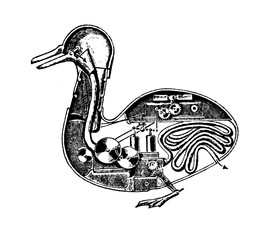
\includegraphics[scale=0.8]{imagenes/digestingduck.jpg}
	\caption{Año 1738. Autómata con forma de pato de Jacques de Vaucanson.} \label{fig:duck}
\end{figure}

\noindent Con la Revolución Industrial y el desarrollo de la tecnología comenzaron a crearse robots más complejos con motores y energía eléctrica, con formas humanoides. En el año 1917, Karel Čapek publicó Rossum's Universal Robots, que dio lugar al término \textit{robot}; además, Isaac Asimov, escribió un libro, ``Runaround'' (``Círculo vicioso''), en 1942, en el que aparecía por primera vez la palabra \textit{robótica} y se establecían las leyes de los robots. \\

\noindent Joe Engleberger junto con George Devol, lanzaron al mercado el primer robot que se comercializaría (\ref{fig:unim}), con lo que Joe Engleberger comenzó a ser considerado el padre de la robótica, ya que creó la primera empresa dedicada a este campo, \textit{Unimation} con robots preparados para la industria en los años 1950 y 1960. \\

\begin{figure}[!h]
	\centering % si queremos la imagen centrada
	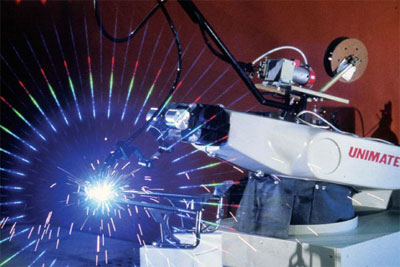
\includegraphics[scale=0.5]{imagenes/unimate.jpg}
	\caption{Año 1956. Robot industrial Unimate.} \label{fig:unim}
\end{figure}

\noindent Siguieron construyéndose robots utilizados en distintas ramas, como la industria, el espacio o destinados a la interacción con el ser humano. \\
\noindent Entre algunos impulsores de la robótica, se encuentra Rodney Brooks \cite{rodneybrooks}, el director y presidente de Rethink Robotics; fue un estudiante de matemáticas que recibió un Ph.D. en informática y que más tarde ejerció de profesor de robótica. Fundó el laboratorio de Ciencias de la Computación e Inteligencia Artificial y cofundó iRobot. En 2008 fundó la empresa Rethink Robotics.

\subsubsection{Actualidad}
\label{actualidad}
\noindent La evolución del desarrollo de robots ha permitido que estos trabajen en muchas áreas, como la industria, permitiendo una más rápida adaptación al cambio, así como un trabajo más preciso y con menos errores. Es frecuente a día de hoy decir que los robots generan desempleo, sin embargo, no existen para sustituir a una persona, sino para realizar aquellos trabajos en los que la repetición de procesos y la necesaria cualidad de que se hagan de forma rápida abundan. Cabe decir que muchos de estos trabajos suelen ser incluso peligrosos para las personas \cite{tadele2014safety}, ya que es probable que con la reiteración que supone el realizar estas tareas, el humano se equivoque, cuando un robot no lo hace \cite{brown1994human}. \\
\noindent Puesto que la robótica está obteniendo una gran presencia en la actualidad, es necesario que la sociedad se adapte a este nuevo paradigma, generando nueva formación y empleo de más valor añadido, como por ejemplo ingenieros industriales, ingenieros de automatización, programadores, etc. Además, conforme este proceso se haga más complejo, se hará necesaria la supervisión continuada por parte de especialistas, técnicos, etc. \\

\begin{figure}[H]
	\centering % si queremos la imagen centrada
	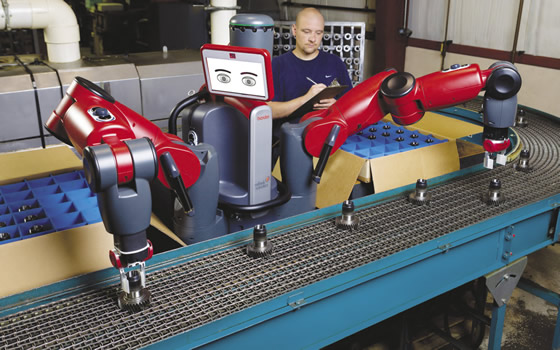
\includegraphics[scale=0.4]{imagenes/bpersona.jpeg}
	\caption{Baxter trabajando cerca de una persona.}
\end{figure}

\noindent En cuanto a Baxter, es un robot con dos brazos robóticos que, a parte de ser un robot seguro \cite{reardon2015towards} y que puede trabajar con personas como se verá en próximas secciones, no es tan caro. Según RobotWorx \cite{robots}, una compañía centrada en robótica de alta calidad a bajo precio, un robot industrial nuevo consistente en un sólo brazo robótico puede llegar a costar entre 50000 y 80000 dólares, sin incluir periféricos de aplicación específicos, con los que el precio puede aumentar hasta los 150000 dólares. En cambio, Baxter cuesta 35000 dólares incluyendo un año de garantía y un año de actualizaciones software, además de las pinzas y la bomba de vacío. \\

\noindent Estos robots industriales en principio tienen este precio, pero después es necesario añadir el coste de las infraestructuras que los rodeen para mantener a los humanos seguros. Generalmente son más difíciles de programar mientras que Baxter no requiere tanta experiencia y puede programarse para realizar varias tareas rápidamente. 


